%%%%%%%%%%%%%%%%%%%%%%%%%%%%%%%% 
\section{The Slow-Control System} 
\label{sec:detectors-fd-alt-dcs}

The slow-control system for the far detector is designed  to
monitor the detector operation conditions, in particular, the following physical
quantities inside the tank:
\begin{itemize}
 \item temperatures (with platinum resistors),
 \item pressures (with commercial piezoelectric sensors),
 \item LAr levels (with custom-made capacitive sensors and electronics), and
 \item deformations of materials (with resistive strain gauges).
\end{itemize} 

In addition, the slow-control system provides the hardware
infrastructure needed to monitor traces of O$_2$, N$_2$ and H$_2$O
impurities in the tank, to monitor and control the high- and
low-voltage power supplies, heaters, lighting system and cryogenic
video system. It will also interface to the cryogenic system and to
the motorized system that adjusts the position of each Charge Readout
Plane (CRP).


The design of the slow-control system is part of a
continued, progressive prototyping effort aimed at developing a
control system dedicated to multi-kiloton LAr dual-phase detectors. It
has been designed in the framework of the LAGUNA-LBNO design study and
 the WA105 experiment. WA105 represents a first, fully engineered,
implementation of this design, which can be extrapolated to larger
detector scales. The design also benefited from the successful example
and the expertise developed in the context of the ArDM
experiment\cite{Badertscher:2013ygt} which is currently operating a
LArTPC for dark matter searches in an underground laboratory (LSC,
Spain).

The slow-control system introduces the use of National Instruments
Compact RIO (Reconfigurable Input Output) modules for acquisition of
all the physical quantities of interest.  Figure~\ref{fig:NI_proto}
shows a rack prepared for the WA105 3$\times$1$\times$1~m$^3$
prototype that is ready to be tested at CERN.
\begin{cdrfigure}[Slow Control prototype rack]{NI_proto}{The rack is a  prototype of the entire Control System; it  embeds modules for resistive 
temperature sensors, pressure  sensors, strain gauges, liquid argon level  meters, control for  heaters. On the upper part a redundant 24 V power supply 
provides fault tolerant power to the National Instrument controller and modules.  Calibration of modules and sensors is ongoing.}
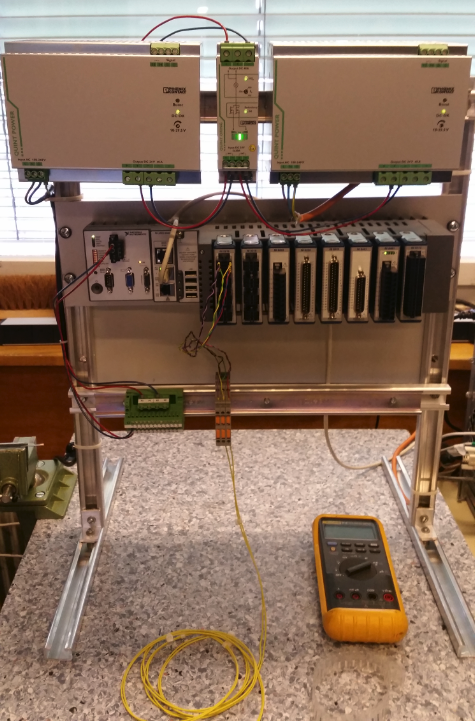
\includegraphics[scale=0.4, angle=0]{rack_2.jpg}
\end{cdrfigure}


The entire slow-control system of the WA105 demonstrator will be
managed through a single LabView interface\cite{WA105_SREP} which
will provide access to all the sensors, control the actuators and
provide the platform for the video monitoring system both inside and
outside the tank.  Supervisory software will be implemented in the
CERN UNICOS (UNified Industrial Control System)
framework~\cite{unicos} to provide the operator interface for the
monitoring of all the physical quantities and the handling of alarms.

As discussed in Section~\ref{sec:detectors-fd-ref-ov}, the
charge-readout system is implemented via CRP modules of
3$\times$3~m$^2$. Each CRP is an independent detector, hence its
instrumentation can also be treated as independent. A complete list of
the sensors planned for use in both the 3$\times$3 m$^2$ DUNE CRP
module and and the 3$\times$1$\times$1~m$^3$ WA105 prototype is
provided in Figure~\ref{fig:sc_sensors}.
\begin{cdrfigure}[Dual-phase slow control sensors]{sc_sensors}
{List of the slow control sensors for the 3$\times$1$\times$1~m$^3$ WA105 prototype and far detectors CRP}
 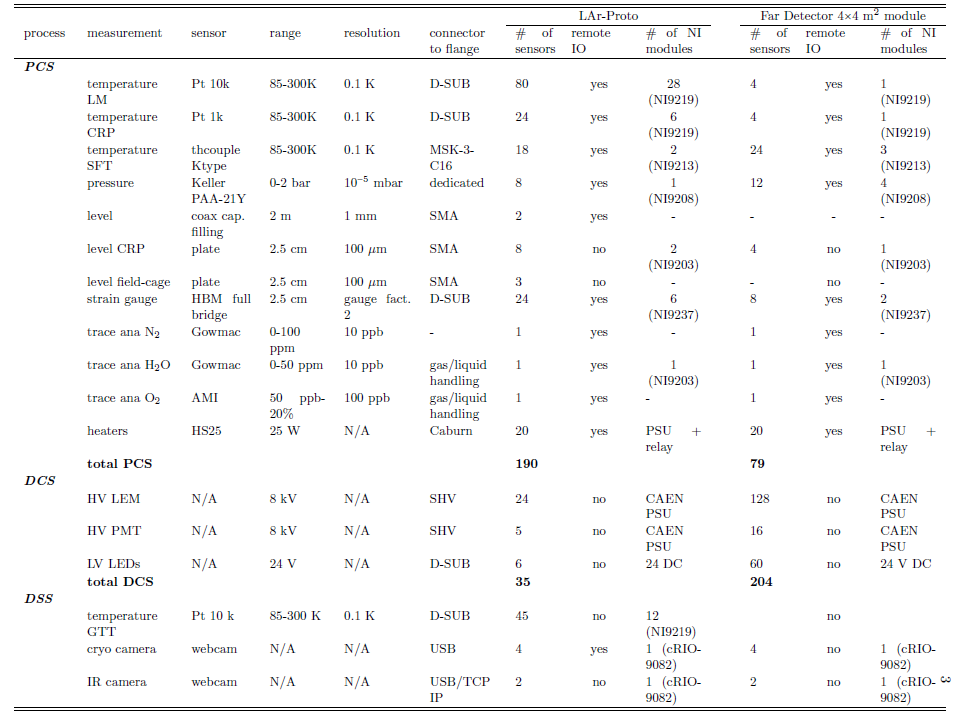
\includegraphics[scale=0.7, angle=0]{sc_table.png} 
 \end{cdrfigure}

The number of sensors for the far detector CRP is extrapolated from
the number for the prototype and is not yet final but it should be
considered as an upper limit. The sensor instrumentation of the
3$\times$1$\times$1~m$^3$ WA105 prototype has also led to the design
of a custom Slow-Control Feedthrough (SCFT), based on the use of
weldable connectors for high vacuum (see
Figure~\ref{fig:SC_flange}). A specific SCFT for the DUNE
3$\times$3~m$^2$ CRP would be based on this design.
\begin{cdrfigure}[Slow control feedthroughs]{SC_flange}{The 3 SCFTs providing 
weldable connectors for all the instrumentation inside the 3$\times$1$\times$1~m$^3$  WA105 tank. 
The number of sensors per module in the DUNE far detector will be drastically 
reduced with respect to this WA105 prototype.}
  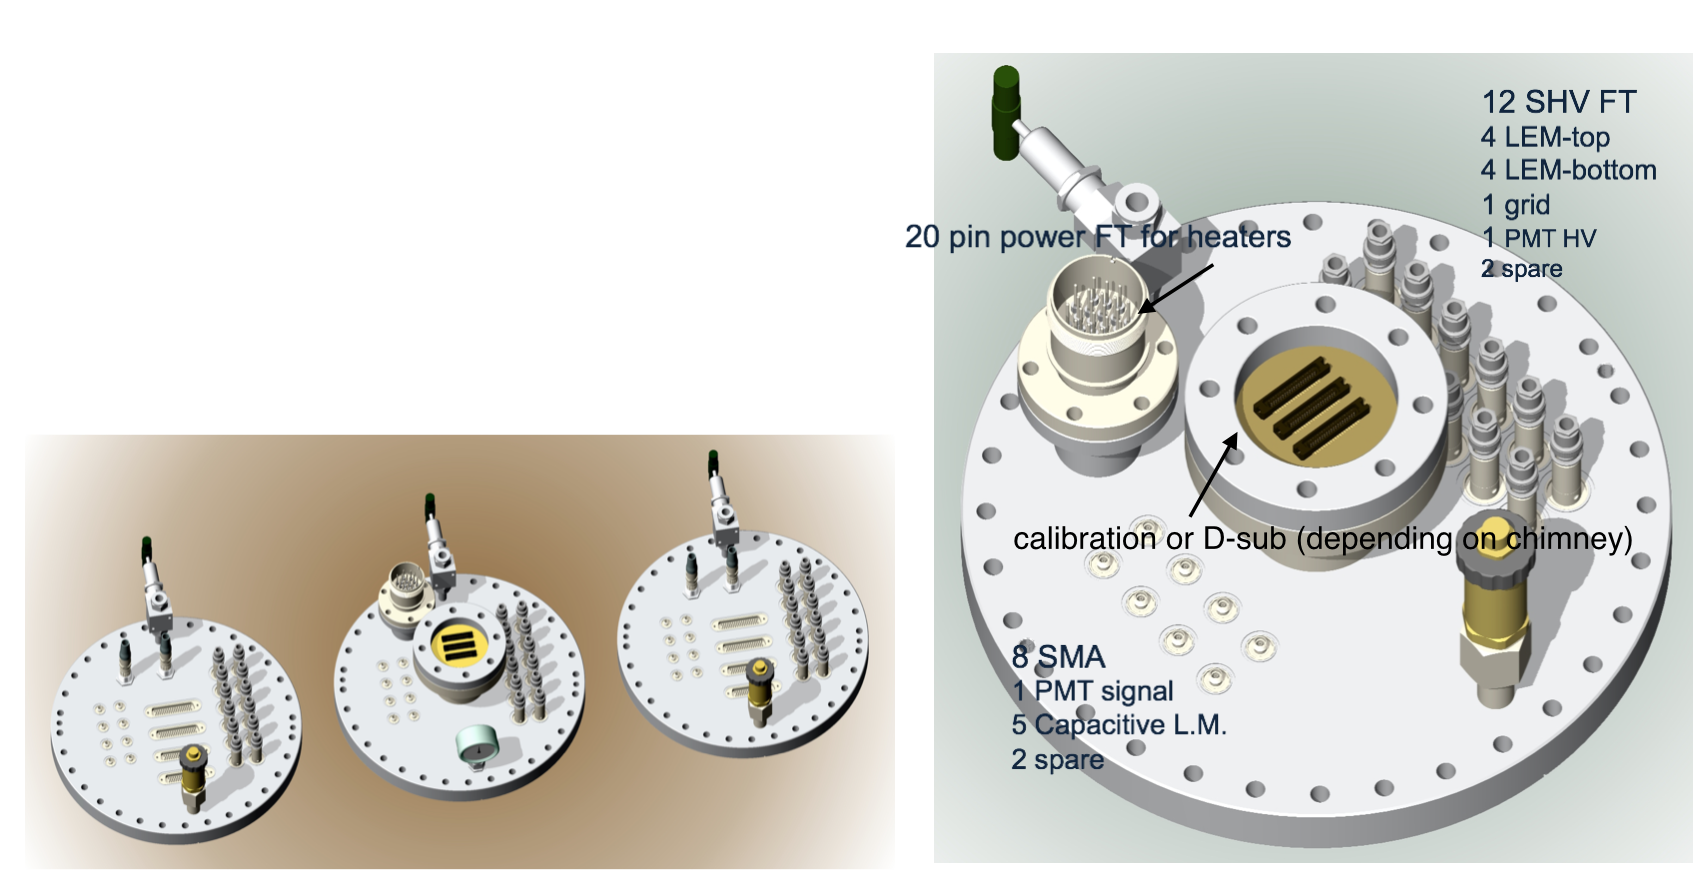
\includegraphics[scale=0.52, angle=0]{SC_flange.png}
 \end{cdrfigure}
